
\section{Results}

For each graph, the blue line corresponds to the time taken by the generate-and-test method and the orange line to the time taken by the FO method. When a result is not in the graph, that means that the execution of the program was interrupted for insufficient memory. For example, the times for the generate-and-test for the yes-instance for $q1$ for the db sizes granter than 1 million are absent.

\begin{figure}[h]
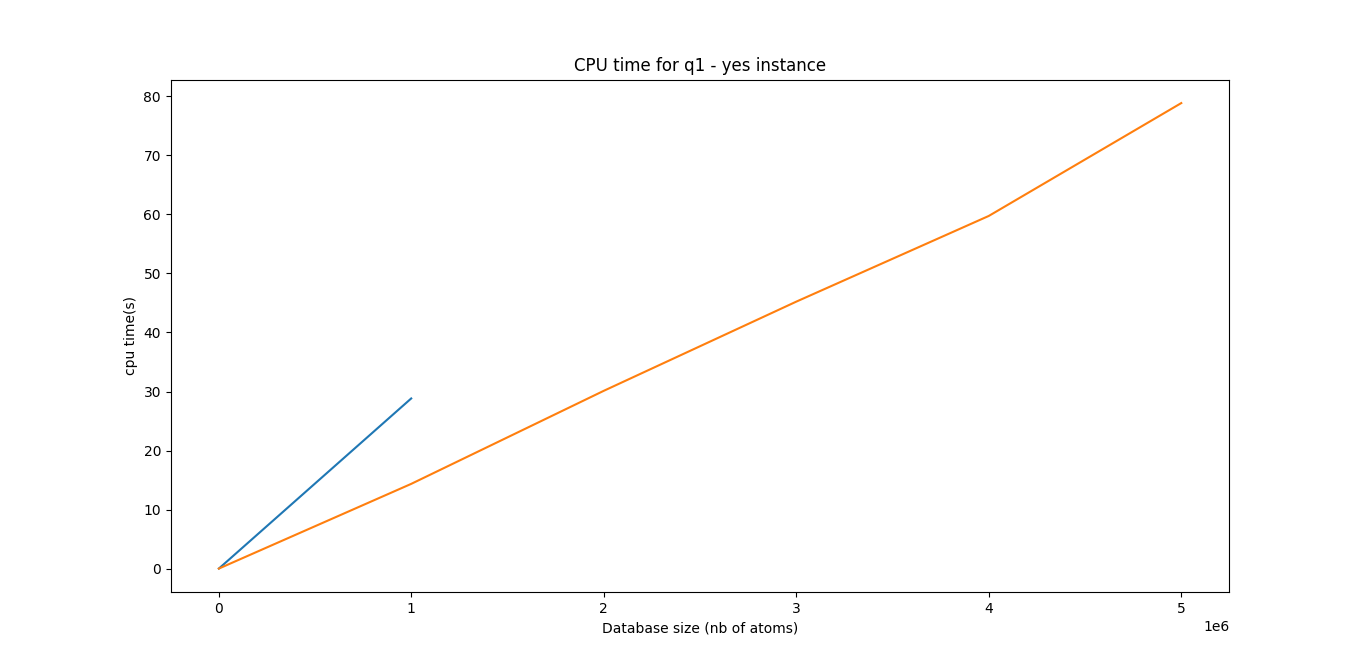
\includegraphics[width=\textwidth]{time_q1_yesinstance.png}
\centering
\end{figure}

\begin{figure}[h]
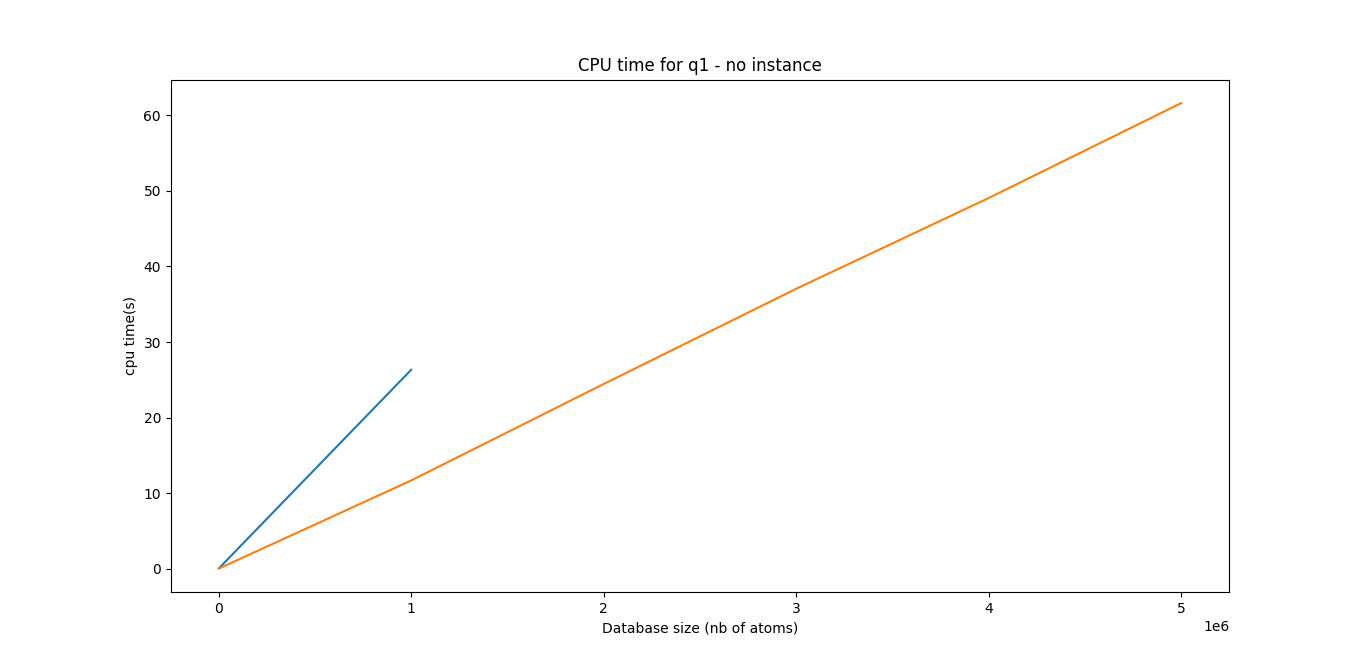
\includegraphics[width=\textwidth]{time_q1_noinstance.png}
\centering
\end{figure}

\begin{figure}[h]
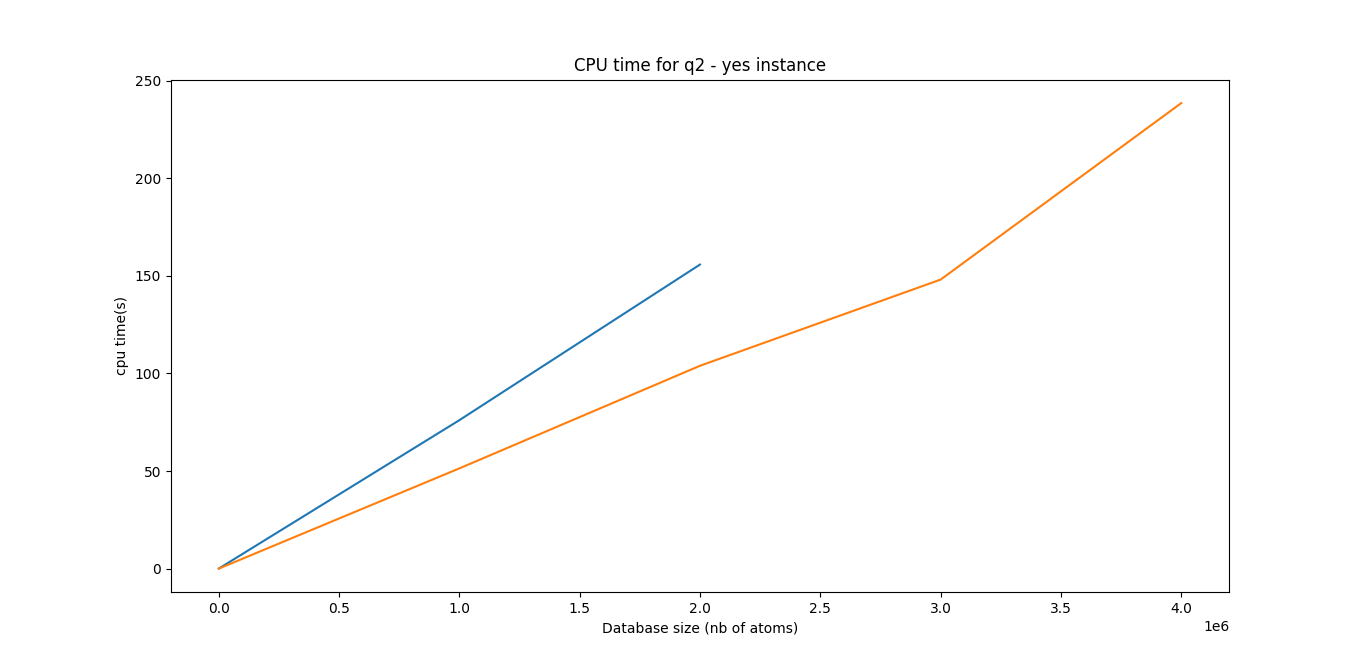
\includegraphics[width=\textwidth]{time_q2_yesinstance.png}
\centering
\end{figure}

\begin{figure}[h]
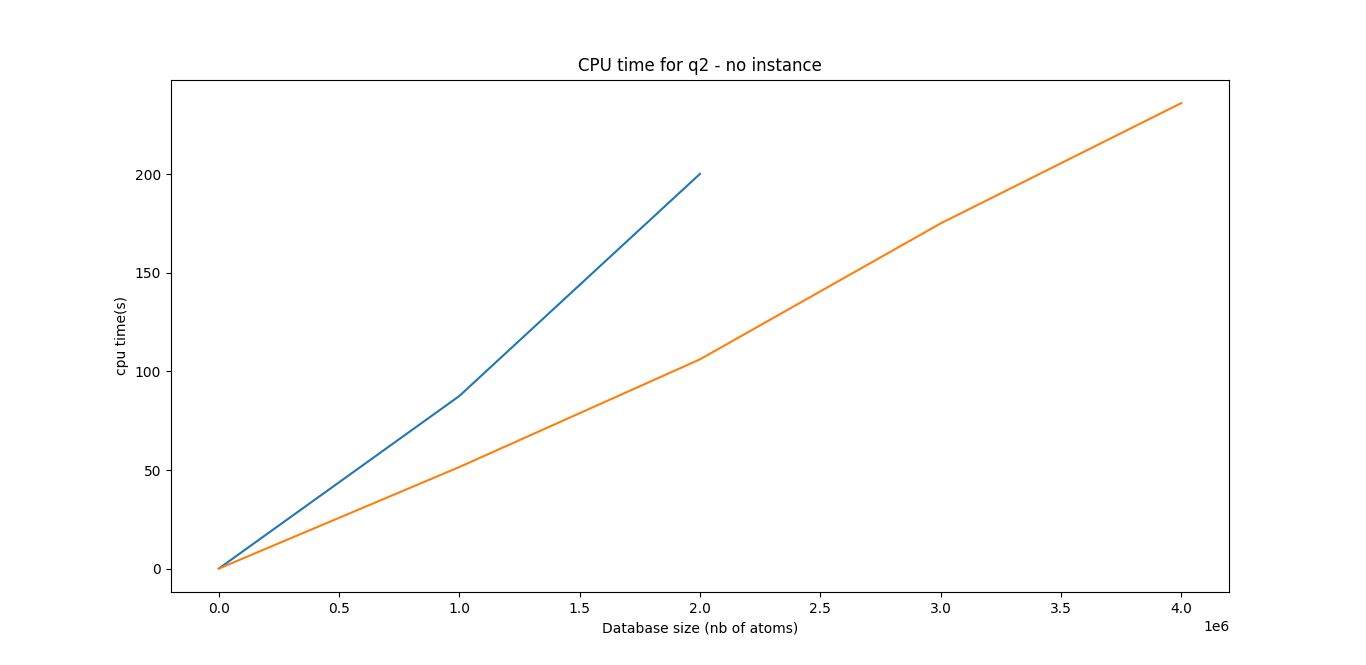
\includegraphics[width=\textwidth]{time_q2_noinstance.png}
\centering
\end{figure}

\begin{figure}[h]
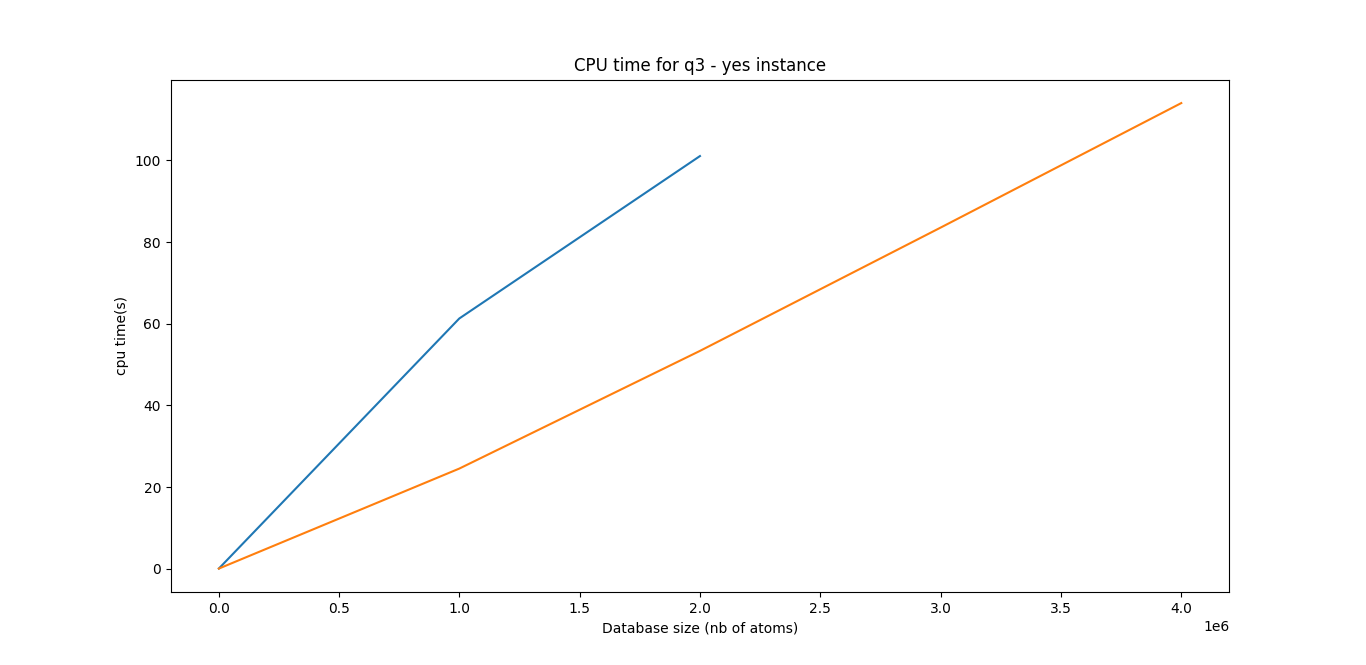
\includegraphics[width=\textwidth]{time_q3_yesinstance.png}
\centering
\end{figure}

\begin{figure}[h]
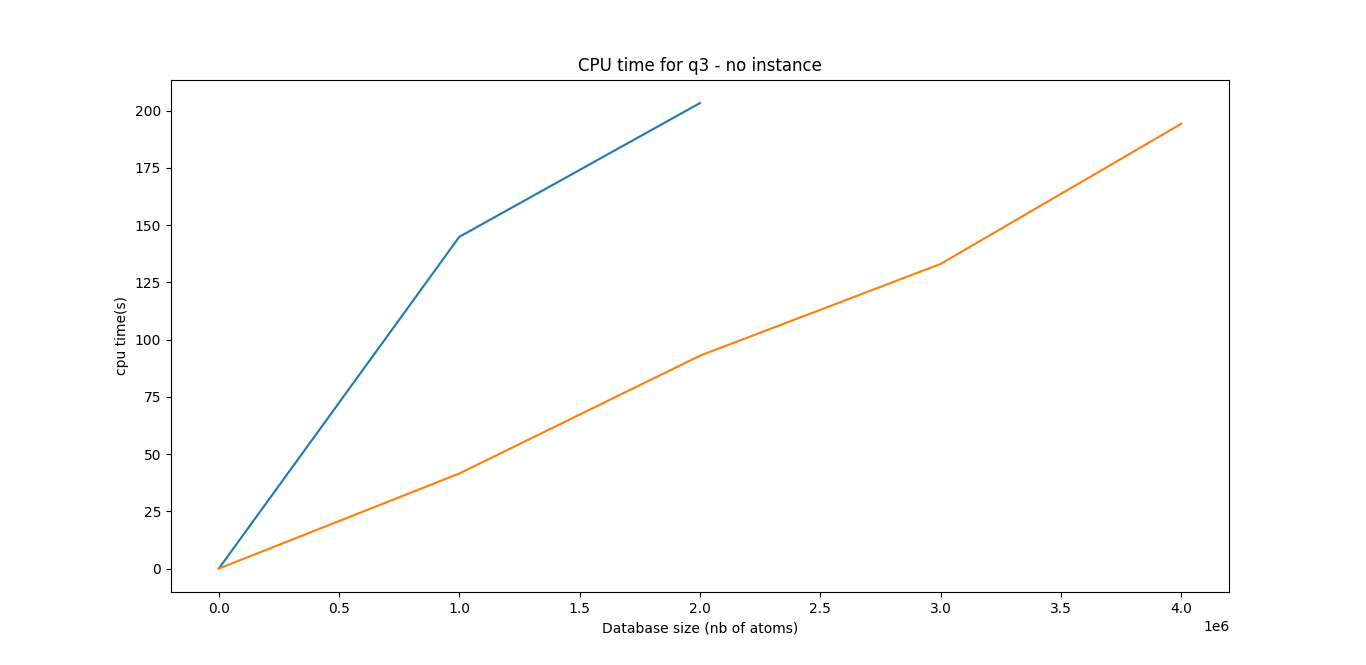
\includegraphics[width=\textwidth]{time_q3_noinstance.png}
\centering
\end{figure}

\textcolor{red}{We see that the fo rewriting leads to better results, in terms of cpu time, that the generate-and-test method.}

\section{Conclusion}

This project was very fun